\documentclass[12pt]{article}

\usepackage{graphicx}
\usepackage[utf8]{inputenc}
\usepackage[english,russian]{babel}
\usepackage[pdftex,unicode]{hyperref}
\usepackage[margin=15mm,left=2cm]{geometry}
\usepackage{indentfirst}
\usepackage{amsbib}

\sloppy
\clubpenalty=999
\widowpenalty=9999

% This is all for formatting and making the Table of Contents according to 
% spec. Don't play with it.
\makeatletter
\renewcommand\l@section[2]{%
    \ifnum \c@tocdepth >\z@
        \addpenalty\@secpenalty
        \addvspace{1.0em \@plus\p@}%
        \setlength\@tempdima{1.5em}%
        \begingroup
        \parindent \z@ \rightskip \@pnumwidth
        \parfillskip -\@pnumwidth
        \leavevmode \bfseries
        \advance\leftskip\@tempdima
        \hskip -\leftskip
#1\nobreak\ 
        \leaders\hbox{$\m@th\mkern \@dotsep mu\hbox{.}\mkern \@dotsep mu$}
    \hfil \nobreak\hb@xt@\@pnumwidth{\hss #2}\par
        \endgroup
    \fi}
\makeatother

\title{Верхние оценки параметра treewidth для класса предикатных схем}
\author{Василевская И.\,Ю.}
\date{\today}

\begin{document}
    \begin{titlepage}
        \begin{center}
            Московский Государственный Университет им. Ломоносова\\
            Факультет Вычислительной Математики и Кибернетики\\
            Кафедра Математической Кибернетики\\
            магистратура, отделение <<МММ СБИС>>\\[6cm]

            \large {Василевская Инесса Юрьевна}\\
            \LARGE \textbf {Верхние оценки одного параметра для класса предикатных схем}\\[0.8cm]
            \large \emph {Курсовая работа}\\[5.0cm]

            \begin{flushright}
                \large
                \begin{minipage}{0.40\textwidth}
                    \begin{flushleft}
                        \emph{Научный руководитель:}\\к.ф.м.н М.\,С.~Шуплецов
                    \end{flushleft}
                \end{minipage}
            \end{flushright}

            \vfill
            Москва\\
			2012
        \end{center}
    \end{titlepage}

\setcounter{page}{2}

\section{Введение}
\label{beginning}
В ряде работ (\cite{Shu09}, \cite{Shu11}) рассматривается задача синтеза для специального класса дискретных управляющих систем ~--
класса предикатных схем, который обобщает некоторые традиционные классы схем. Данные схемы строятся из предикатных элементов
и обладают рядом отличий от схем из других классов (например, направление протекания сигналов не является фиксированным).
Указанные выше работы в основном посвящены исследованию асимптотики функции Шеннона в классе предикатных схем,
 получению асимптотических оценок высокой степени точности и вопросам моделирования предикатными схемами схем из традиционных классов.

В силу особенностей класса предикатных схем, при его рассмотрении могут возникать вопросы,
нетипичные для традиционных классов. Так, к примеру, довольно любопытен вопрос функционирования предикатных схем с точки зрения оценки времени, которое нужно затратить для
вычисления конкретной схемы. 
В данной работе в качестве меры <<быстрой вычислимости>>\footnote{в англоязычной литературе употребляется термин tracktability}
 был выбран так называемый параметр \textit{ширины декомпозиции}~-- максимального числа вершин в узле дерева, 
которое можно оптимально построить по заданной предикатной схеме. Во многих работах (например, \cite{CSP10}, \cite{Gott10}, \cite{Prosc89}) было 
показано, что задачи, которые можно переформулировать в терминах Constraint Satisfaction Problem, быстро вычислимы, если ширина декомпозиции графа ограничений 
(constraint graph) ограничена сверху константой. 
Так как задача функционирования предикатных схем естественным образом представляется как задача CSP с булевыми ограничениями,
 вопрос <<быстрой вычислимости>> заданного предиката в конкретном базисе сводится к нахождению такого способа синтеза, 
 при котором результирующая схема будут иметь ограниченный параметр ширины декомпозиции
\footnote
{В англоязычных источниках известного как treewidth. В силу отсутствия общепринятого перевода, автор вводит 
понятие <<ширины декомпозиции>>}.

\section{Основные определения}
Ниже приведены формальные определения используемых в работе понятий.

\subsection{Предикатные схемы}

В настоящей работе определение предикатных схем будет дано по аналогии с \cite{Shu11}.

\textbf{Опредение}.
\textit{Схемой из предикатных элементов} или \textit{предикатной схемой в базисе $\Pi$} назовем помеченный
неориентированный двудольный граф следующей структуры:

\begin{itemize}
\item каждая вершина из первой доли помечена некоторым множеством символов из алфавита X и/или 
множеством символов из алфавита Y. 
Алфавит $X$ соответствует \textit{входным} переменным предиката, а $Y$ ~-- его внутренним переменным, 
т.е. переменным, возникающим непосредственно в процессе вычисления; 

\item каждая вершина второй доли помечена некоторым символом $\pi_i$ из множества $\Pi$ и 
соединена $k$ ребрами, пронумерованными числами $1, ..., k$, с вершинами из первой доли.
\end{itemize}

Вершины из первой доли будем называть \textit{узлами} схемы, а вершины из второй доли ~-- её \textit{предикатными элементами}. 
Узлы схемы, соединенные ребрами с предикатным элементом, будем называть полюсами этого элемента, 
а узлы, соответствующие входным переменным, ~-- полюсами схемы.
При этом считается, что узел является $j$-м полюсом предикатного элемента и соответствует 
его $j$-ой переменной, если соединяющее их ребро имеет номер $j$. Полюс схемы, которому приписано 
более одной входной переменной, называется кратным полюсом этой схемы. 

Будем считать элементарной такую предикатную схему, которая состоит либо из изолированной полюсной вершины, 
либо только из одного предикатного элемента $\pi_i$, $1 < i < k$, где $k$ ~-- число полюсов указанного элемента.

В тех случаях, когда это не вызывает разночтений, 
не будем различать узел схемы и переменную, 
символ которой приписан данной вершине, а также предикатный элемент и сам предикат, отвечающий этому элементу. 
Также, для удобства, в некоторых случаях будем использовать упрощенное описание предикатной схемы, 
опуская пометки дуг и некоторых внутренних вершин. 

\subsection{Функционирование предикатных схем}
Функционирование предикатного элемента с $k$ полюсами задается его характеристической функцией от $k$ переменных, 
связанных с указанными полюсами, и определяется тем, что предикатный элемент находится в допустимом состоянии на тех и 
только тех наборах значений этих переменных, на которых данная функция равна 1. 

Предикатная схема $\Sigma$ находится в допустимом состоянии на заданном наборе значений её полюсных переменных тогда и только тогда, 
когда существует такой набор значений внутренних переменных схемы, на котором все предикатные элементы схемы находятся в допустимых состояниях. 
Если же указанного набора значений внутренних переменных не существует, то считается, что схема находится в недопустимом состоянии на 
заданном наборе значений её полюсных переменных.

Предполагается, что предикатная схема $\Sigma$ реализует предикат $\pi$ от её полюсных переменных, если множество допустимых наборов $\pi$ 
совпадает с множеством тех наборов, на которых $\Sigma$ находится в допустимом состоянии. 
При этом схемы будем называть эквивалентными, если они реализуют равные предикаты. 
Отметим, что элементарная предикатная схема, состоящая из изолированной полюсной вершины, реализует тождественно истинный предикат.
 Будем считать также, что тождественно истинный (соответственно тождественно ложный)
 предикат реализуется любой предикатной схемой без входных полюсов, 
которая имеет непустое (соответственно пустое) множество допустимых состояний.

В общем случае граф предикатной схемы может содержать несколько компонент связности. 
В дальнейшем, будем считать, что схема не содержит компонент связности, 
которые не имеют полюсных узлов и для которых существует хотя бы один допустимый набор, так как такие компоненты не влияют на функционирование схемы.

Суперпозицией двух предикатных схем, не имеющих общих вершин и пометок, 
будем называть их объединение с возможным отождествлением группы полюсов этих схем, 
которое сопровождается приписыванием новой (``объединенной'') вершине либо 
некоторого подмножества переменных данной группы, либо ``новой'' внутренней переменной.
 При этом частными случаями суперпозиции являются следующие операции:
\begin{itemize}
\item переименование полюсной переменной схемы

\item введение фиктивной полюсной переменной схемы

\item проекция или снятие полюсной переменной схемы

\item отождествление двух полюсных переменных схемы
\end{itemize}

\subsection{Шефферов базис}

\textbf{Теорема (Критерий полноты для предикатных схем)}. Система из $B$ предикатов является полной $\iff$
она не лежит целиком ни в одном из 7 предполных классов: $T_0, T_1, SM, SL, $. \cite{Shu11} (УТОЧНИТЬ ФОРМУЛИРОВКУ!!!)

\textbf{Следствие.} $\pi =  $ ~-- полная система, $\pi$~--- Шефферов предикат.

Ниже приведен пример построения предикатной схемы в Шеффером базисе, реализующей $z=\overline{x \oplus y}$.

\begin{figure}[htb]
\centering
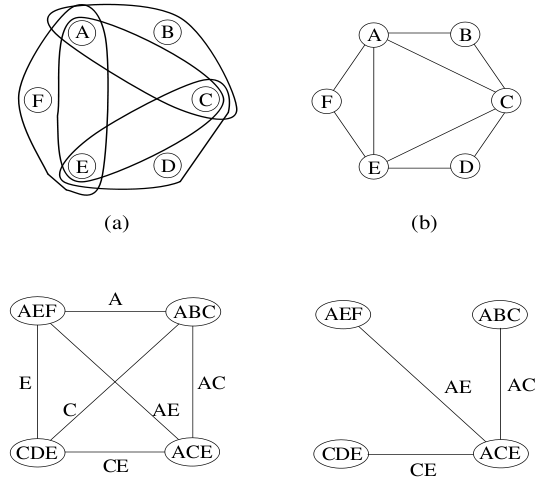
\includegraphics[width=0.01\textwidth]{constraint_graph.png}
\caption{$z=\overline{x \oplus y}$ в Шефферовом базисе}
\label{fig:sheff}
\end{figure}

\subsection{Обобщенная задача выполнимости}

Формально, \textit{обобщенная задача выполнимости (CSP)}\footnote{Constraint Satisfaction Problem} 
~--- это тройка $<X,D,C>$, где $X$ ~-- набор переменных, $D$ ~-- область определения (домен допустимых значений), 
а $C$ ~-- набор ограничений. Ограничения имеют вид $<t, R_n>$, где $t$ ~--- кортеж из $n$ переменных множества $X$, 
$R_n$ ~-- заданное на $D$ отношение арности $n$. 
Решением задачи CSP является набор значений переменных $X$, который удовлетворяет всем ограничениям из $C$. 

Так, например, задачу 3-ВЫП можно рассматривать как обобщенную задачу выполнимости над булевым доменом, с 
состоящим лишь из отношений-конъюнкций множеством ограничений.

В ряде работ рассматривалась вычислительная сложность задачи CSP. Несмотря на то, что в общем случае задача CSP
принадлежит классу NP, при введении определенных ограничений на множество $C$ или структуру так называемого
графа ограничений\footnote{constraints graph}, существуют быстрые алгоритмы нахождения решения. 
Так, например, в \cite{Shaeffer78} показано, 
что, в тех случаях, когда множество $C$ имеет определенный вид, существуют полиномиальные алгоритмы нахождения решения.
В данной работе будет внимательно рассмотрен второй подход, связанный с исследованием структурных особенностей 
графа ограничений. 

\subsection{Граф ограничений}
Графическим представлением задачи CSP является граф ограничений. 
Существуют несколько вариантов представления графа ограничений\cite{CSP10}\footnote
{в виде гиперграфа, primal-constraint графа, dual-constraint графа}, однако в
данной работе будет использован dual-constraint граф. Строится он следующим образом: 
\begin{itemize}
\item Каждая вершина графа ограничений соответствует одному ограничению; сама вершина помечается множеством переменных, 
входящих в ограничение.
\item Если множества пометок двух вершин имеют непустое пересечение, то между вершинами проводится ребро, которое помечается 
множеством общих переменных.
\end{itemize}

Часто вместо dual-constraint graph рассматривают join-tree constraint graph(JTCG), который получается из первого удалением 
``дублирующих информацию'' ребер. Пусть между двумя вершинами существует путь, 
в пометки каждого ребра которого входит множество $A$. Тогда ребра, которые лежат на других путях между этими вершинами, 
с множеством пометок в точности $A$, называются ``дублирующими информацию'', и их можно убрать без изменения функционирования. 

В дальнейшем, под графом ограничений будет имется в виду join-tree constraint graph.

На рисунке \ref{fig:constraint_graph} приведены примеры соответствующих графов.

\begin{figure}[htb]
\centering
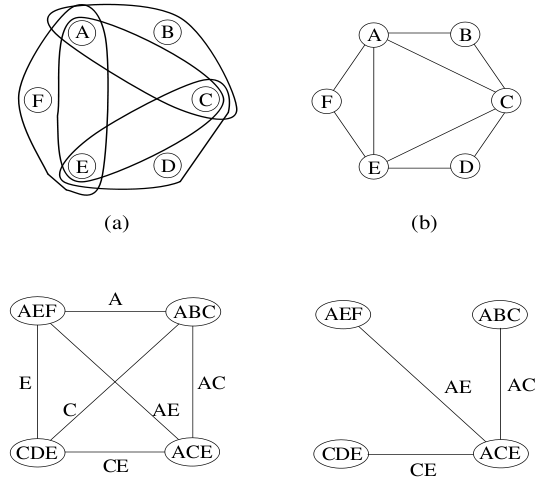
\includegraphics[width=0.50\textwidth]{constraint_graph.png}
\caption{Представления графа ограничений: а~-- гиперграф, b~-- primal graph, c~-- dual graph, d~-- join-tree }
\label{fig:constraint_graph}
\end{figure}


\subsection{Ширина декомпозиции}
\textbf{Определение}. Пусть $R = (X, D, C)$~--- задача CSP. \textit{Декомпозицией $R$} 
будем называть тройку $< T, X, \Psi >$, где $T = (V, E)$~-- дерево, $\chi$, $\psi$ ~-- 
размечающие функции, ставящие в соответствие каждой вершине $v \subseteq V$ два множества, $\chi(v) \subseteq X$
и $\psi(v) \subseteq C$, что выполняются:
\begin{itemize}
\item Каждому ограничению $R_i \in C$, соответствует как минимум одна вершина $v \in V$,
такая что $R_i \in \phi(v)$, и область определения $R_i \subseteq \chi(v)$.
\item (Свойство связности). 
Каждой переменной $X_i \in X$, соответсвует множество ${v \in V |X_i \in \chi(v)}$, порождающее
связное поддерево дерева $T$. 
\end{itemize}

\textbf{Определение.}
\textit{Шириной декомпозиции $ < T, X, \Psi >$} называется $tw = \max_{v \in V}{|\chi(v)| - 1}$.
Шириной декомпозиции задачи CSP~-- $\min_{all~decompositions}{tw}$.


\textbf{Теорема}. В случае, когда $tw \leq const$, 
решение можно найти за полиномиальное от числа отношений время. \cite{CSP10}

\subsection{Forbidden graph characterization, k-outerplanar graphs}
При нахождении верхних оценок будет использоваться классификация графов по запрещенным минорам.
Особое внимание будет уделено классу внепланарных графов.

\textbf{Определение.}
Hеориентированный граф $H$ называется \textit{минором графа} $G$, если $H$
является подграфом графа $G$, или может быть получен из подграфа графа $G$ применением операции реберного стягивания.

\textbf{Определение.}
A 1-outerplanar embedding of a graph is the same as an outerplanar embedding. 
For k > 1 a planar embedding is k-outerplanar if removing the vertices on the outer
face results in a (k - 1)-outerplanar embedding. A graph is k-outerplanar if it has a 
k-outerplanar embedding.

\textbf{Теорема (признак внешнепланарности графа).}
Граф $G$ является внешнепланарным $\iff$ $G$ не содержит миноров $K_4$ и $K_{2,3}$\cite{Diestel00}.

\begin{figure}[htb]
\centering
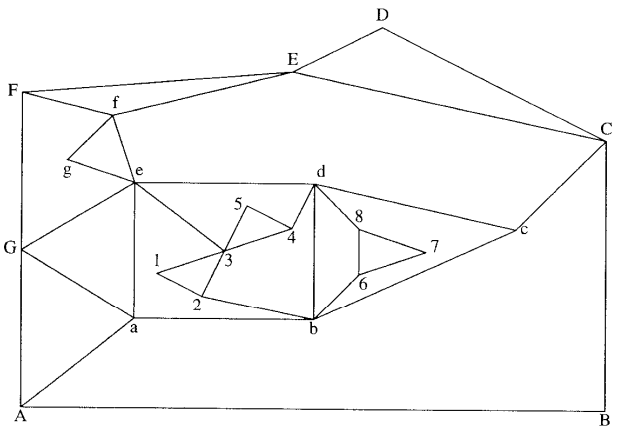
\includegraphics[width=0.50\textwidth]{outerplanar.png}
\caption{Пример 3-внепланарного графа.}
\label{fig:outerplanar_graph}
\end{figure}

\textbf{Теорема.}
Пусть $G$~-- $k$-внепланарный граф. Тогда $tw(G) \leq 3k-1.$\cite{Boedlander96}

\subsection{Число скрещиваний графа}

\textbf{Определение.} \textit{Числом скрещиваний графа}\footnote{graph crossing number} называют 
минимальное число реберных пересечений, необходимое для укладки графа в плоскость.

\label{ZarankTheorem}
\textbf{Теорема (Заранкевича)} Число скрещиваний полного двудольного $K_{n,m}$ графа $\leq$
$\lfloor \frac{n}{2} \rfloor \lfloor \frac{n-1}{2} \rfloor \lfloor \frac{m}{2} \rfloor \lfloor \frac{m-1}{2} \rfloor$.
\cite{Zarank54}
\section{Основная часть}
\subsection{Сведение задачи вычисления предикатной схемы к задаче нахождения решения задачи CSP}
Как было отмечено в \S \ref{beginning}, задачу функционирования предикатной схемы можно свести к задаче нахождения решения в CSP. 

Пусть предикатная схема $\Sigma$ имеет $m$ входных переменных $x_1, \ldots , x_m$, 
$k$ внутренних переменных $y_1, \ldots , y_k$ и $n$ предикатных элементов $B = \pi_1, \dots , \pi_n$. 
Тогда, для определения функционирования этой схемы нужно найти валидные значения внутренних переменных на всех $2^{m}$
наборах входных переменных. 

Нетрудно видеть, что эта задача может быть сведена к задаче CSP $<X, D, C>$ следующим образом:
$X$ = $X \bigcup Y$, $D = [0, 1]$, $C = B$. Аналогично поиску функционирования предикатной схемы, 
будут поставлены $2^m$ задач нахождения решения, перед началом вычисления которых переменные $x_1, \ldots , x_m$ 
во всех ограничениях, их содержащих, будут забиты соответствующими значениями $\alpha_1, \ldots , \alpha_n$.

В обеих моделях, сложность вычислений в худшем случае, при применении алгоритма поиска 
с откатом без памяти, требует $2^m * (2^k)^N$ операций, где $N$ ~-- количество предикатов (ограничений) 
в схеме (графе ограничений).

\subsection{Связь графа предикатной схемы и графа ограничений}

\textbf{Утверждение 1.} Если граф предикатной схемы планарен, то граф ограничений тоже будет планарен.

Это нетрудно показать, приведя алгоритм построения графа ограничений по заданной предикатной схеме. 
Пусть дана предикатная схема, уложенная на плоскости без пересечений. Чтобы построить соответствующий ей граф
ограничений\footnote{Join Tree Constraint Graph}, нужно сделать следующее:
\begin{itemize}
\item Каждой предикатной вершине $\pi_i$, смежной с вершинами-переменными $x_1, ... , x_k$, поставить в соответствие
ограничение $c_i$, определенное на множестве $x_1, ..., x_k$.
\item Если какая-то переменная разделялась лишь двумя предикатами, то в графе ограничений
проводится ребро между соответствующими этим предикатам ограничениями; ребро помечается общей переменной.
\item Если какая-то переменная разделялась более чем двумя предикатами, то эти предикаты соединяются 
реберной цепью, как показано на рисунке \ref{fig:induced_to_constraint}. Ребра помечаются общей переменной.
\end{itemize}

Нетрудно видеть, что, после вышеописанных преобразований, получается планарный join tree constraint graph.

\begin{figure}[htb]
\centering
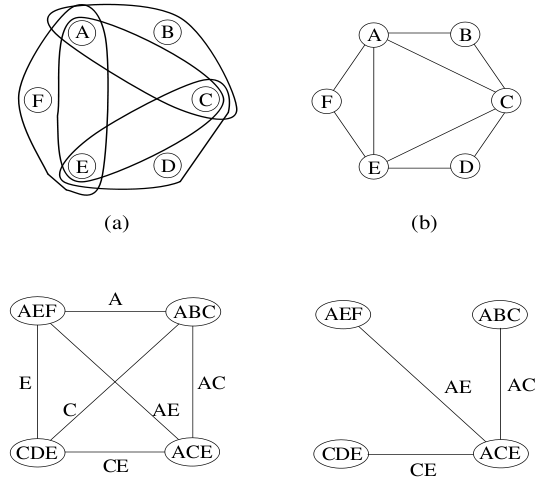
\includegraphics[width=0.01\textwidth]{constraint_graph.png}
\caption{Отображение некоторых подграфов предикатной схемы в подграфы графа ограничений}
\label{fig:induced_to_constraint}
\end{figure}
!!!КАРТИНКУ СЮДА БЫСТРО!!!

\textbf{Утверждение 2.} Если граф предикатной схемы не планарен, то граф ограничений может быть как планарным, 
так и не планарным.
Примеры приведены на \ref{fig:planar_non_planar}. 

\begin{figure}[htb]
\centering
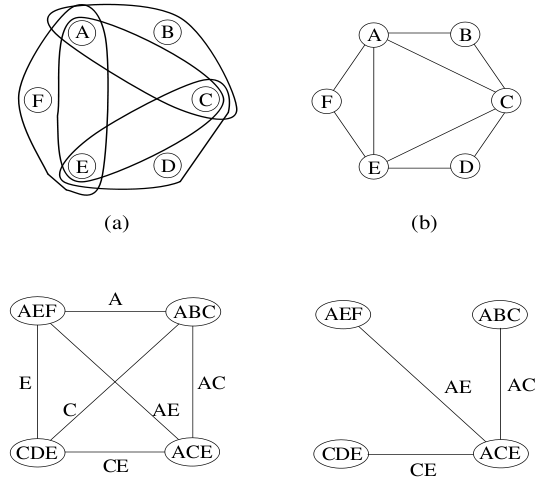
\includegraphics[width=0.01\textwidth]{constraint_graph.png}
\caption{$K_{3,3}$ и $K_{6,9}$}
\label{fig:planar_non_planar}
\end{figure}

\textbf{Теорема 1.} В Шефферовом базисе любой непланарный граф можно сделать планарным, 
добавив $\leq \frac{27}{8}*k(k-1)$ предикатов, где $k$~-- максимальная степень вершины-переменной.

\textbf{Доказательство.} Пусть дан не планарный граф предикатной схемы в Шефферовом базисе. 
Тогда, при укладке его на плоскость, по \ref{ZarankTheorem}, будет не более 
$\lfloor \frac{3}{2} \rfloor \lfloor \frac{2}{2} \rfloor \lfloor \frac{k}{2} \rfloor \lfloor \frac{k-1}{2} \rfloor$
$\leq \frac{3}{8}*k(k-1)$ реберных пересечений, где $k$~-- максимальная степень вершин из вершинной доли.
Заменяя каждое пересечение по схеме на рисунке \ref{fig:make_planar},
граф предикатной схемы можно сделать планарным,
увеличив сложность в смысле числа предикатов не более чем на $\frac{27}{8}*k(k-1)$, $\otimes$.
\begin{figure}[htb]
\centering
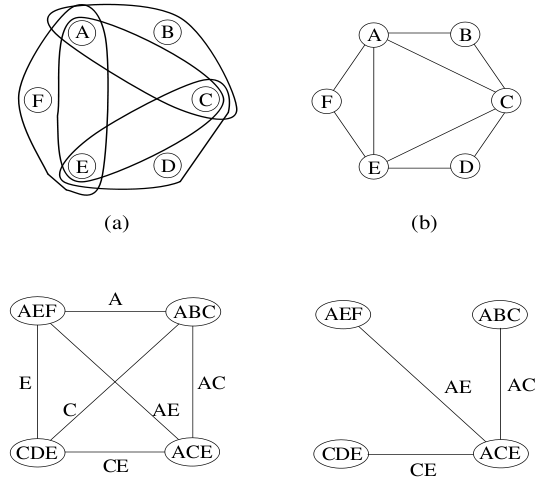
\includegraphics[width=0.01\textwidth]{constraint_graph.png}
\caption{Избавление от пересечения с помощью трех элементов $z=\overline{x \oplus y}$}
\label{fig:make_planar}
\end{figure}

\textbf{Следствие 1.} В Шефферовом базисе граф ограничений можно сделать планарным, увеличив число ограничений 
на не более чем $\frac{27}{8}*k(k-1)$.

\begin{figure}[htb]
\centering
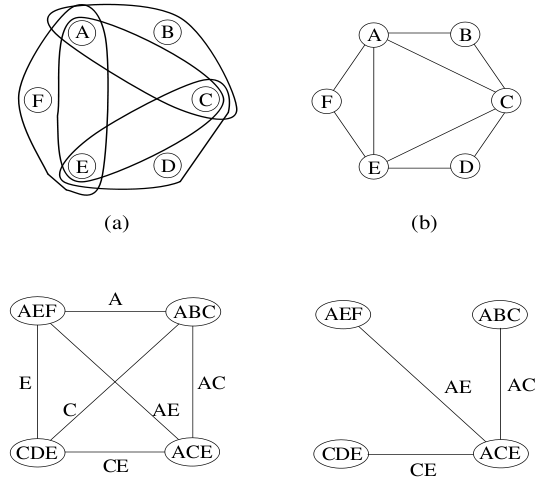
\includegraphics[width=0.01\textwidth]{constraint_graph.png}
\caption{Подграф графа предикатной схемы после избавления от одного пересечения.}
\label{fig:make_planar_induced}
\end{figure}

\begin{figure}[htb]
\centering
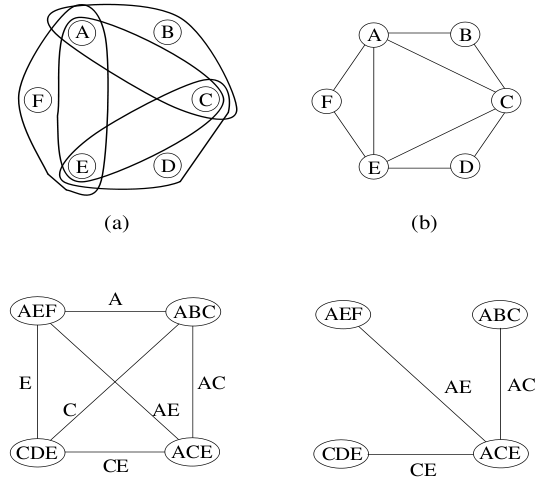
\includegraphics[width=0.01\textwidth]{constraint_graph.png}
\caption{Подграф графа ограничений после избавления от одного пересечения.}
\label{fig:make_planar_constraint}
\end{figure}

Заметим, что, при таком преобразовании, степень внешнепланарности графа предикатной схемы возрастает на 1, а 
степень внешнепланарности графа ограничений остается неизменной.

% Список цитируемой литературы
\clearpage
\addcontentsline{toc}{section}{Список цитируемой литературы}
\thebibliography{99}
\RBibitem{Shu09}
    \by М.~С.~Шуплецов
    \paper Оценки высокой степени точности для сложности предикатных схем в~некоторых базисах
    \inbook Физико-математические науки
    \serial Уч\"eн. зап. Казан. гос. ун-та. Сер. Физ.-матем. науки
    \yr 2009
    \vol 151
    \issue 2
    \pages 173--184
    \publ Изд-во Казанского ун-та
    \publaddr Казань
    \mathnet{http://mi.mathnet.ru/uzku760}

\bibitem{Shu11}Методы синтеза и оценки сложности схем, построенных из элементов предикатного типа, диссертация

\bibitem{CSP10} Handbook of Constraint Programming, ISBN 9780444527264; 2010 г.

\bibitem{Shaeffer78} Schaefer, Thomas J. (1978). 
``The Complexity of Satisfiability Problems''. STOC 1978. pp. 216–226. doi:10.1145/800133.804350.

\bibitem{Zarank54} Zarankiewicz, K. "On a Problem of P. Turán Concerning Graphs." Fund. Math. 41, 137-145, 1954. 

\bibitem{Prosc89} Arnborg, S.; Proskurowski, A. (1989), 
``Linear time algorithms for NP-hard problems restricted to partial k-trees'',
Discrete Applied Mathematics 23 (1): 11–24, doi:10.1016/0166-218X(89)90031-0.

\bibitem{Gott10} 
Georg Gottlob, Reinhard Pichler, and Fang Wei. 2010. Bounded treewidth as a key to tractability of knowledge representation and reasoning. Artif. Intell. 174, 1 (January 2010), 105-132. DOI=10.1016/j.artint.2009.10.003 http://dx.doi.org/10.1016/j.artint.2009.10.003

\bibitem{Diestel00}
Diestel, Reinhard (2000), Graph Theory, Graduate Texts in Mathematics, 
173, Springer-Verlag, ISBN 0-387-98976-5.

\bibitem{Boedlander96}
H. L. Bodlaender, A linear-time algorithm for finding 
tree-decompositions of small
treewidth, SIAM J. Comput. 25 (1996), 1305–1317


\endthebibliography

\end{document}
